\documentclass{tufte-book}

% For revision control
\usepackage{rcs-multi}
\rcsid{$Id$}
\rcsid{$Header$}
\rcskwsave{$Author$}
\rcskwsave{$Date$} 
\rcskwsave{$Revision$}
\rcsRegisterAuthor{devangel}{Dennis J. Evangelista}
\rcsRegisterAuthor{taliaym}{Talia Y. Moore}

% Use some useful packages
\usepackage[pdftex]{graphicx}
\setkeys{Gin}{width=\linewidth,totalheight=\textheight,keepaspectratio}
%\usepackage[usenames,dvipsnames]{color}
\usepackage{color}
\usepackage{siunitx}
\usepackage{makeidx}
\makeindex

% PDF metadata
\usepackage{hyperref}
\hypersetup{pdftitle={Comparative Biomechanics}}
\hypersetup{pdfauthor={at least D. Evangelista and Talia Y. Moore}}
\hypersetup{pdfsubject={biology}}
\hypersetup{pdfkeywords={biomechanics}}
%\hypersetup{colorlinks=true,citecolor=Violet,linkcolor=Blue,urlcolor=Red}
\hypersetup{colorlinks}

% References in Tufte inline style
% use \cite commands
% also appear collected at the end of the book
%\usepackage{doi}
\renewcommand*{\doi}[1]{\href{http://dx.doi.org/\detokenize{#1}}{doi:\detokenize{#1}}}

% Get chapter numbers
\setcounter{secnumdepth}{1}

% For nicely typeset tabular material
\usepackage{booktabs}

% Prints the month name (e.g., January) and the year (e.g., 2008)
\newcommand{\monthyear}{%
  \ifcase\month\or January\or February\or March\or April\or May\or June\or
  July\or August\or September\or October\or November\or
  December\fi\space\number\year
}

% Use AMS math
\usepackage{amsmath}
\usepackage{amsthm} % Use AMS theorem environments
\theoremstyle{plain}
\newtheorem{thm}{Theorem}[chapter]
\newtheorem{lem}[thm]{Lemma}
\newtheorem{prop}[thm]{Proposition}
\newtheorem*{cor}{Corollary}
\theoremstyle{defninition}
\newtheorem{defn}{Definition}[chapter]
\newtheorem{conj}{Conjecture}[chapter]
\newtheorem{example}{Example}[chapter] % DE added
\newtheorem{exercise}{Exercise}[chapter] % DE added
\newtheorem{demo}{Demonstration}[chapter] % DE added
\theoremstyle{remark}
\newtheorem*{rem}{Remark}
\newtheorem*{note}{Note}
\newtheorem{case}{Case}

% eqExam for problems (compatible with making exams)
%\usepackage[fortextbook,ftbsolns,forcolorpaper,noseparationrule,useexkv]{eqexam}
% not part of my tex distribution!?

% Commands for Genus species names
\newcommand{\species}[1]{\emph{#1}}

% Formatting wish list:
% Cute quotations and pictures for each chapter?  - use Tufte-latex defaults
% Problems/exercises - would prefer to have something able to be made into exams? 






% Book metadata
\title{Comparative Biomechanics}
\author{Dennis Evangelista and Talia Y.\ Moore}
\publisher{Starfleet Academy Press, San Francisco, CA}

\begin{document}

\frontmatter
\maketitle
\rcsid{$Id$}
\rcsid{$Header$}
\rcskwsave{$Author$}
\rcskwsave{$Date$} 
\rcskwsave{$Revision$}




\newpage
\begin{fullwidth}
~\vfill
\thispagestyle{empty}
\setlength{\parindent}{0pt}
\setlength{\parskip}{\baselineskip}
Copyright \copyright\ \the\year\ \thanklessauthor

\par\smallcaps{Published by \thanklesspublisher}

\par\smallcaps{fun-url-here.com}

\par\texttt{hg clone \url{ssh://hg@bitbucket.org/devangel77b/superbook}}

\par This work is licensed under the Creative Commons \smallcaps{Attribution-NonCommercial-NoDerivs 3.0 Unported} License. To view a copy of this license, visit \url{http://creativecommons.org/licenses/by-nc-nd/3.0/} or send a letter to Creative Commons, 444 Castro Street, Suite 900, Mountain View, California, 94041, USA. \index{license}

\par\textit{First printing, \monthyear}
\end{fullwidth}

\cleardoublepage
\thispagestyle{empty}
\vspace*{\stretch{1}}
\hfill\begin{minipage}[t]{0.66\textwidth}
\raggedright
Dedication here.  To those about to rock, we salute you.
\end{minipage}
\vspace*{\stretch{3}}
\clearpage

\rcsid{$Id$}
\rcsid{$Header$}
\rcskwsave{$Author$}
\rcskwsave{$Date$} 
\rcskwsave{$Revision$}

\chapter*{Preface}
%\addcontentsline{toc}{chapter}{Preface}

%% THIS BIT MOVED TO CH WHY BIOMEX
%Biomechanics is the study of motion and how it affects biological systems. It's a discipline at the interface of evolutionary biology, developmental biology, materials science, engineering, physics, and mathematics. Integrating methodology from so many different disciplines, each with their unique lingo for the same ideas, can be confusing. We aim to provide a crash course in the methods used to study much of biomechanics, with an optional explanation of how each was derived, and ultimately to show how biomechanics can be used to answer questions meaningful to evolutionary, ecological, or medical study.

% Not sure "motion" is the defining thing about biomechanics.  It's the application of mechanics
% - physics and engineering methods for understanding motion, force, strength, flow, heat and mass
% transfer, etc - to things that are alive.  However it's not just that - it's understanding the 
% biological contexts - historical, ecological, behavioral, etc. There is a Wainwright quote about
% structure without function is a corpse; function without structure is a ghost.  

% Notion that interdisciplinary is hard and need to get people speaking each other's languages is good. 

% "Crash course" sounds like we're short changing them.  

This is a book about biomechanics based on the notes and coverage of four courses:  Berkeley's \emph{Biomechanics of Organisms}\sidenote{Integrative Biology 135}, Harvard's \emph{Comparative Biomechanics}\sidenote{Organismic and Evolutionary Biology 273}, Friday Harbor Lab's \emph{Biomechanics}\sidenote{number}, and MIT's \emph{2.183}\sidenote{Neural Control of Movement}.  

Each of these was a pleasure to take, but they all lacked a single, coherent textbook to which students could refer.  This is probably to be expected, considering how multidisciplinary biomechanics is.  However, it seems necessary for a text to provide general information to bridge the leap between Powerpoint slides and lecture notes (which go so fast) and the full-strength undiluted papers from the primary literature (which can be quite daunting), and to give example problems illustrating how to think through some of the more engineering aspects of the subject; more so when one considers how multidisciplinary the students are.

Having been teaching assistants for the Berkeley and Harvard versions of this class, we hope the examples and problems here will prove helpful.  We also hope that the existence of this document in an open, editable\sidenote{To clone this book, visit \url{ssh://hg@bitbucket.org/devangel77b/superbook}} and possibly reflowable form\sidenote{Currently \LaTeX, hopefully to later include .ePub, for all you iPad and Kindle fans.} will ease the load on graduate students too often asked to scan and revise a print of a scan of a print of scan.  Clickers be damned, but some digital technologies, appropriately applied, can be useful.

Also, it is our sincere hope this will be accessible and affordable to as wide a group of students as possible.  This is quite important in days where annual tuition hikes of 30\% are not unheard of, the latest editions of glossy color print textbooks cost upwards of \$90.00, universities make advertising deals with publishers\cite{Asimov:2012}, and university administrators make upwards of \$800,000 a year. 

% This is a comment.  If Talia can read this she is an honorary MIT dork.
% I can read it. If Dennis can see this then I'm really an honorary MIT dork.
% Only if you stop bathing. 

\rcsid{$Id$}
\rcsid{$Header$}
\rcskwsave{$Author$}
\rcskwsave{$Date$} 
\rcskwsave{$Revision$}

\chapter*{Acknowledgements}

We thank a bunch of people.
\tableofcontents
\listoffigures
\listoftables





\mainmatter
\rcsid{$Id$}
\rcsid{$Header$}
\rcskwsave{$Author$}
\rcskwsave{$Date$} 
\rcskwsave{$Revision$}
\rcsRegisterAuthor{devangel}{Dennis J. Evangelista}

\chapter{Some preliminaries}
\section{What is biomechanics?}
\section{Why study biomechanics?}
\section{Engineering and physics}
\section{Evolution}
\section{Who's who?}
\section{Scaling}
\section{Problems}


%\bibliographystyle{apalike}
%\bibliography{whybiomex}

\part{Background and theory}
% For revision control
\rcsid{$Id$}
\rcsid{$Header$}
\rcskwsave{$Author$}
\rcskwsave{$Date$} 
\rcskwsave{$Revision$}
\rcsRegisterAuthor{devangel}{Dennis J. Evangelista}



\chapter{Solids}
% chapter author here?
% chapter abstract here?
Solids are evil. That is why the Dominion wages war against them \citep{Son-of-Moog:2488}.

\section{History of solid aggression in the Gamma Quadrant}
\section{Weaknesses of solids and Dominion anti-solid strategies and tactics}
\begin{figure}[h!]
 \label{jaculus}
 \centering
  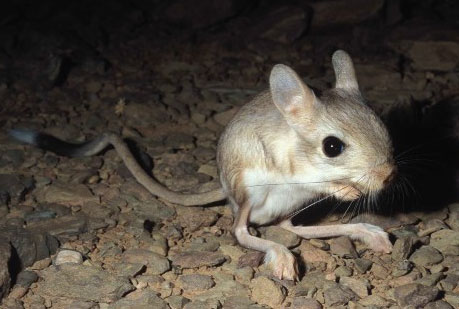
\includegraphics[width=0.5\textwidth]{ch-solids/figures/jaculus.jpg}
 \caption{The Dipodid \species{Jaculus jaculus}, believed to resemble the ancestor of crown-group Voortaidae.}
\end{figure}


\bibliographystyle{apalike}
\bibliography{references/ch-solids}

\rcsid{$Id$}
\rcsid{$Header$}
\rcskwsave{$Author$}
\rcskwsave{$Date$} 
\rcskwsave{$Revision$}
\rcsRegisterAuthor{devangel}{Dennis J. Evangelista}

\chapter{Fluids}
\label{ch:fluids}
%\index{subjects}{fluid|(}
\index{fluid|(}
\chauthor{Dennis Evangelista}{Department of Integrative Biology, University of California, Berkeley}


\section{What is a fluid?}
%\index{subjects}{fluid!definition}
\index{fluid!definition}
This is an example citation \citep{Janeway:2392}.

\section{Fluid properties}
%\index{subjects}{fluid!properties}
%\index{subjects}{fluid|)}
\index{fluid!properties}
\index{fluid|)}

\section{Example equation and table}

\begin{equation}
u_1 A_1 = u_2 A_2
\label{eq:continuity}
\index{equation!continuity}
\end{equation}

\begin{table}
\caption{Hello world}
\begin{center}
\begin{tabular}{cc}
one & two \\
three & four \\
\end{tabular}
\end{center}
\end{table}

%\nocite{*}
\bibliographystyle{apalike}
\bibliography{references/ch-fluids.bib}

\part{Measurement and modeling techniques}


\appendix
\rcsid{$Id$}
\rcsid{$Header$}
\rcskwsave{$Author$}
\rcskwsave{$Date$} 
\rcskwsave{$Revision$}

\chapter{Test appendix}
\label{app:test}
%\index{subjects}{Appendix}
\index{Appendix}

\section{Useful data}
%\index{subjects}{useful!data}
\index{useful!data}

\section{Useful equations}
%\index{subjects}{useful!equations}
\index{useful!equations}



\setcounter{secnumdepth}{-1} % Don't number bibliography and index
\bibliographystyle{jeb}
\nobibliography{references/main}

\pagestyle{plain}
%\addcontentsline{toc}{chapter}{Index}
\printindex
\end{document}
